\documentclass[a4paper,UKenglish,cleveref, autoref, thm-restate]{lipics}
%This is a template for producing LIPIcs articles. 
%See lipics-v2021-authors-guidelines.pdf for further information.
%for A4 paper format use option "a4paper", for US-letter use option "letterpaper"
%for british hyphenation rules use option "UKenglish", for american hyphenation rules use option "USenglish"
%for section-numbered lemmas etc., use "numberwithinsect"
%for enabling cleveref support, use "cleveref"
%for enabling autoref support, use "autoref"
%for anonymousing the authors (e.g. for double-blind review), add "anonymous"
%for enabling thm-restate support, use "thm-restate"
%for enabling a two-column layout for the author/affilation part (only applicable for > 6 authors), use "authorcolumns"
%for producing a PDF according the PDF/A standard, add "pdfa"

%\graphicspath{{./graphics/}}%helpful if your graphic files are in another directory

% The macro file
% Imported packages
%\usepackage[utf8x]{inputenc}
\usepackage{amsmath}
\usepackage{amsfonts}
\usepackage{amssymb}
\usepackage[svgnames]{xcolor} % Provides better colors with upper cases
\usepackage{agda} % The Agda package to input Agda code
%\usepackage[right]{lineno} % Allows to number lines
\setlength\linenumbersep{-8pt} % Moves left by 8pt the line numbers
\usepackage{xargs} % Allows to create better commands
\usepackage{tikz}
\usepackage{xspace}
%\usepackage{graphicx}
\usetikzlibrary{positioning,backgrounds,arrows,automata}
\usepackage{multicol}
\usepackage{mdframed}

% Comments macros
\newcommand{\cath}[1]{\textcolor{Blue}{CD : #1}}
\newcommand{\amelie}[1]{\textcolor{Red}{AL : #1}}
\newcommand{\mathieu}[1]{\textcolor{Green}{MM : #1}}

% Special words macros
\newcommand{\coq}{\textsc{Coq}\xspace}
\newcommand{\agda}{\textsc{Agda}\xspace}
\newcommand{\lagda}{\texttt{lagda}\xspace}
\newcommand{\haskell}{\textsc{Haskell}\xspace}
\newcommand{\datatypes}{datatypes\xspace}
\newcommand{\Datatypes}{Datatypes\xspace}
\newcommand{\datatype}{datatype\xspace}
\newcommand{\libName}{\textsc{LibNDT}\xspace}
\newcommand{\linear}{\textsc{LNDT}\xspace}
\newcommand{\linears}{\textsc{LNDTs}\xspace}
\newcommand{\linearsFull}{linked nested \datatypes\xspace}

% URL macros
\newcommand{\gitURL}{\url{https://bitbucket.org/MonsieurO/nested/}}

% Mapping of unknown characters
\DeclareUnicodeCharacter{8759}{\ensuremath{::}}
\DeclareUnicodeCharacter{955}{\ensuremath{\lambda}}
\DeclareUnicodeCharacter{969}{\ensuremath{\omega}}

% Other macros
\AgdaNoSpaceAroundCode % The name says it all
\renewcommandx*{\hrulefill}[2][1=0.3mm,2=0pt] % A \rule with parameterized positioning
    {\leavevmode \leaders \hbox to 1pt{\rule[#2]{1pt}{#1}} \hfill \kern 0pt}

\setlength{\mathindent}{.8 cm}%

% Macros to define paragraphs, either the first of the section, or the next one
% This is useful because lipics treats paragraphs like sections, which is not always what we want
\newcommand{\myfirstparagraph}[1]{\noindent\textbf{#1} --}%
\newcommand{\myparagraph}[1]{\vspace{.2cm}\myfirstparagraph{#1}}%

\tikzset{
    node distance=5mm and -9mm, %Caractéristiques sur les noeuds
    boite/.style={ %Caractéristiques sur le styles des boites
        fill=blue!50!cyan!70,
        draw,
        align=center,
        font=\footnotesize\bfseries,
        text=white,
    },
    boite coins ronds/.style={ %Caractéristiques sur les boites
        boite,
        rounded corners=3pt
    },
    boite circulaire/.style={ %Caractéristiques sur les boites circulaires
        boite,
        circle
    },
    fleche/.style={ %Caractéristiques sur les flèches
        line cap=round,
        -latex,
        line width=0.25mm,
	    draw=blue!50!cyan!30,
	},
	grosse fleche/.style={ %Caractéristiques sur les grosses flèches
	    fleche,
	    line width=1mm
	},
}

% The file containing Agda code converted into latex commands
\newcommand{\imports}{
\begin{code}%
\>[0]\AgdaKeyword{module}\AgdaSpace{}%
\AgdaModule{AgdaTypes}\AgdaSpace{}%
\AgdaKeyword{where}\<%
\\
%
\\[\AgdaEmptyExtraSkip]%
\>[0]\AgdaKeyword{open}\AgdaSpace{}%
\AgdaKeyword{import}\AgdaSpace{}%
\AgdaModule{Agda.Primitive}\<%
\\
\>[0]\AgdaKeyword{open}\AgdaSpace{}%
\AgdaKeyword{import}\AgdaSpace{}%
\AgdaModule{Data.Product}\AgdaSpace{}%
\AgdaKeyword{using}\AgdaSpace{}%
\AgdaSymbol{(}\AgdaOperator{\AgdaFunction{\AgdaUnderscore{}×\AgdaUnderscore{}}}\AgdaSpace{}%
\AgdaSymbol{;}\AgdaSpace{}%
\AgdaOperator{\AgdaInductiveConstructor{\AgdaUnderscore{},\AgdaUnderscore{}}}\AgdaSpace{}%
\AgdaSymbol{;}\AgdaSpace{}%
\AgdaFunction{∃}\AgdaSymbol{)}\<%
\\
\>[0]\AgdaKeyword{open}\AgdaSpace{}%
\AgdaKeyword{import}\AgdaSpace{}%
\AgdaModule{Data.Nat}\AgdaSpace{}%
\AgdaKeyword{hiding}\AgdaSpace{}%
\AgdaSymbol{(}\AgdaOperator{\AgdaFunction{\AgdaUnderscore{}⊔\AgdaUnderscore{}}}\AgdaSymbol{)}\<%
\\
\>[0]\AgdaKeyword{open}\AgdaSpace{}%
\AgdaKeyword{import}\AgdaSpace{}%
\AgdaModule{Relation.Binary.PropositionalEquality}\<%
\\
\>[0]\AgdaKeyword{open}\AgdaSpace{}%
\AgdaKeyword{import}\AgdaSpace{}%
\AgdaModule{Function}\<%
\\
\>[0]\AgdaKeyword{open}\AgdaSpace{}%
\AgdaKeyword{import}\AgdaSpace{}%
\AgdaModule{Data.String}\<%
\\
\>[0]\AgdaKeyword{open}\AgdaSpace{}%
\AgdaKeyword{import}\AgdaSpace{}%
\AgdaModule{Data.Sum}\AgdaSpace{}%
\AgdaKeyword{using}\AgdaSpace{}%
\AgdaSymbol{(}\AgdaOperator{\AgdaDatatype{\AgdaUnderscore{}⊎\AgdaUnderscore{}}}\AgdaSpace{}%
\AgdaSymbol{;}\AgdaSpace{}%
\AgdaInductiveConstructor{inj₁}\AgdaSpace{}%
\AgdaSymbol{;}\AgdaSpace{}%
\AgdaInductiveConstructor{inj₂}\AgdaSymbol{)}\<%
\end{code}
}

\newcommand{\exampleList}{
\begin{code}%
\>[0]\AgdaKeyword{data}\AgdaSpace{}%
\AgdaDatatype{List₀}\AgdaSpace{}%
\AgdaSymbol{\{}\AgdaBound{a}\AgdaSymbol{\}}\AgdaSpace{}%
\AgdaSymbol{(}\AgdaBound{A}\AgdaSpace{}%
\AgdaSymbol{:}\AgdaSpace{}%
\AgdaPrimitive{Set}\AgdaSpace{}%
\AgdaBound{a}\AgdaSymbol{)}\AgdaSpace{}%
\AgdaSymbol{:}\AgdaSpace{}%
\AgdaPrimitive{Set}\AgdaSpace{}%
\AgdaBound{a}\AgdaSpace{}%
\AgdaKeyword{where}\<%
\\
\>[0][@{}l@{\AgdaIndent{0}}]%
\>[2]\AgdaInductiveConstructor{[]}\AgdaSpace{}%
\AgdaSymbol{:}\AgdaSpace{}%
\AgdaDatatype{List₀}\AgdaSpace{}%
\AgdaBound{A}\<%
\\
%
\>[2]\AgdaOperator{\AgdaInductiveConstructor{\AgdaUnderscore{}∷\AgdaUnderscore{}}}\AgdaSpace{}%
\AgdaSymbol{:}\AgdaSpace{}%
\AgdaBound{A}\AgdaSpace{}%
\AgdaSymbol{→}\AgdaSpace{}%
\AgdaDatatype{List₀}\AgdaSpace{}%
\AgdaBound{A}\AgdaSpace{}%
\AgdaSymbol{→}\AgdaSpace{}%
\AgdaDatatype{List₀}\AgdaSpace{}%
\AgdaBound{A}\<%
\end{code}
}

\newcommand{\exampleNest}{
\begin{code}%
\>[0]\AgdaKeyword{data}\AgdaSpace{}%
\AgdaDatatype{Nest₀}\AgdaSpace{}%
\AgdaSymbol{\{}\AgdaBound{a}\AgdaSymbol{\}}\AgdaSpace{}%
\AgdaSymbol{(}\AgdaBound{A}\AgdaSpace{}%
\AgdaSymbol{:}\AgdaSpace{}%
\AgdaPrimitive{Set}\AgdaSpace{}%
\AgdaBound{a}\AgdaSymbol{)}\AgdaSpace{}%
\AgdaSymbol{:}\AgdaSpace{}%
\AgdaPrimitive{Set}\AgdaSpace{}%
\AgdaBound{a}\AgdaSpace{}%
\AgdaKeyword{where}\<%
\\
\>[0][@{}l@{\AgdaIndent{0}}]%
\>[2]\AgdaInductiveConstructor{[]}\AgdaSpace{}%
\AgdaSymbol{:}\AgdaSpace{}%
\AgdaDatatype{Nest₀}\AgdaSpace{}%
\AgdaBound{A}\<%
\\
%
\>[2]\AgdaOperator{\AgdaInductiveConstructor{\AgdaUnderscore{}∷\AgdaUnderscore{}}}\AgdaSpace{}%
\AgdaSymbol{:}\AgdaSpace{}%
\AgdaBound{A}\AgdaSpace{}%
\AgdaSymbol{→}\AgdaSpace{}%
\AgdaDatatype{Nest₀}\AgdaSpace{}%
\AgdaSymbol{(}\AgdaBound{A}\AgdaSpace{}%
\AgdaOperator{\AgdaFunction{×}}\AgdaSpace{}%
\AgdaBound{A}\AgdaSymbol{)}\AgdaSpace{}%
\AgdaSymbol{→}\AgdaSpace{}%
\AgdaDatatype{Nest₀}\AgdaSpace{}%
\AgdaBound{A}\<%
\end{code}
}

\newcommand{\exampleBush}{
\begin{code}%
\>[0]\AgdaKeyword{data}\AgdaSpace{}%
\AgdaDatatype{Bush₀}\AgdaSpace{}%
\AgdaSymbol{\{}\AgdaBound{a}\AgdaSymbol{\}}\AgdaSpace{}%
\AgdaSymbol{(}\AgdaBound{A}\AgdaSpace{}%
\AgdaSymbol{:}\AgdaSpace{}%
\AgdaPrimitive{Set}\AgdaSpace{}%
\AgdaBound{a}\AgdaSymbol{)}\AgdaSpace{}%
\AgdaSymbol{:}\AgdaSpace{}%
\AgdaPrimitive{Set}\AgdaSpace{}%
\AgdaBound{a}\AgdaSpace{}%
\AgdaKeyword{where}\<%
\\
\>[0][@{}l@{\AgdaIndent{0}}]%
\>[2]\AgdaInductiveConstructor{[]}\AgdaSpace{}%
\AgdaSymbol{:}\AgdaSpace{}%
\AgdaDatatype{Bush₀}\AgdaSpace{}%
\AgdaBound{A}\<%
\\
%
\>[2]\AgdaOperator{\AgdaInductiveConstructor{\AgdaUnderscore{}∷\AgdaUnderscore{}}}\AgdaSpace{}%
\AgdaSymbol{:}\AgdaSpace{}%
\AgdaBound{A}\AgdaSpace{}%
\AgdaSymbol{→}\AgdaSpace{}%
\AgdaDatatype{Bush₀}\AgdaSpace{}%
\AgdaSymbol{(}\AgdaDatatype{Bush₀}\AgdaSpace{}%
\AgdaBound{A}\AgdaSymbol{)}\AgdaSpace{}%
\AgdaSymbol{→}\AgdaSpace{}%
\AgdaDatatype{Bush₀}\AgdaSpace{}%
\AgdaBound{A}\<%
\end{code}
}

\begin{code}[hide]%
\>[0]\AgdaFunction{TT}\AgdaSpace{}%
\AgdaSymbol{:}\AgdaSpace{}%
\AgdaPrimitive{Setω}\<%
\\
\>[0]\AgdaFunction{TT}\AgdaSpace{}%
\AgdaSymbol{=}\AgdaSpace{}%
\AgdaSymbol{∀}\AgdaSpace{}%
\AgdaSymbol{\{}\AgdaBound{b}\AgdaSymbol{\}}\AgdaSpace{}%
\AgdaSymbol{→}\AgdaSpace{}%
\AgdaPrimitive{Set}\AgdaSpace{}%
\AgdaBound{b}\AgdaSpace{}%
\AgdaSymbol{→}\AgdaSpace{}%
\AgdaPrimitive{Set}\AgdaSpace{}%
\AgdaBound{b}\<%
\end{code}

\newcommand{\lndt}{
\begin{code}%
\>[0]\AgdaKeyword{data}\AgdaSpace{}%
\AgdaDatatype{LNDT}\AgdaSpace{}%
\AgdaSymbol{(}\AgdaBound{F}\AgdaSpace{}%
\AgdaSymbol{:}\AgdaSpace{}%
\AgdaFunction{TT}\AgdaSymbol{)}\AgdaSpace{}%
\AgdaSymbol{\{}\AgdaBound{a}\AgdaSymbol{\}}\AgdaSpace{}%
\AgdaSymbol{(}\AgdaBound{A}\AgdaSpace{}%
\AgdaSymbol{:}\AgdaSpace{}%
\AgdaPrimitive{Set}\AgdaSpace{}%
\AgdaBound{a}\AgdaSymbol{)}\AgdaSpace{}%
\AgdaSymbol{:}\AgdaSpace{}%
\AgdaPrimitive{Set}\AgdaSpace{}%
\AgdaBound{a}\AgdaSpace{}%
\AgdaKeyword{where}\<%
\\
\>[0][@{}l@{\AgdaIndent{0}}]%
\>[2]\AgdaInductiveConstructor{[]}\AgdaSpace{}%
\AgdaSymbol{:}\AgdaSpace{}%
\AgdaDatatype{LNDT}\AgdaSpace{}%
\AgdaBound{F}\AgdaSpace{}%
\AgdaBound{A}\<%
\\
%
\>[2]\AgdaOperator{\AgdaInductiveConstructor{\AgdaUnderscore{}∷\AgdaUnderscore{}}}\AgdaSpace{}%
\AgdaSymbol{:}\AgdaSpace{}%
\AgdaBound{A}\AgdaSpace{}%
\AgdaSymbol{→}\AgdaSpace{}%
\AgdaDatatype{LNDT}\AgdaSpace{}%
\AgdaBound{F}\AgdaSpace{}%
\AgdaSymbol{(}\AgdaBound{F}\AgdaSpace{}%
\AgdaBound{A}\AgdaSymbol{)}\AgdaSpace{}%
\AgdaSymbol{→}\AgdaSpace{}%
\AgdaDatatype{LNDT}\AgdaSpace{}%
\AgdaBound{F}\AgdaSpace{}%
\AgdaBound{A}\<%
\end{code}
}

\newcommand{\tuples}{
\begin{code}%
\>[0]\AgdaFunction{Tuple}\AgdaSpace{}%
\AgdaSymbol{:}\AgdaSpace{}%
\AgdaDatatype{ℕ}\AgdaSpace{}%
\AgdaSymbol{→}\AgdaSpace{}%
\AgdaFunction{TT}\<%
\\
\>[0]\AgdaFunction{Tuple}\AgdaSpace{}%
\AgdaInductiveConstructor{zero}\AgdaSpace{}%
\AgdaSymbol{=}\AgdaSpace{}%
\AgdaFunction{id}\AgdaSpace{}%
\AgdaComment{--\ id\ is\ the\ identity\ function}\<%
\\
\>[0]\AgdaFunction{Tuple}\AgdaSpace{}%
\AgdaSymbol{(}\AgdaInductiveConstructor{suc}\AgdaSpace{}%
\AgdaBound{n}\AgdaSymbol{)}\AgdaSpace{}%
\AgdaBound{A}\AgdaSpace{}%
\AgdaSymbol{=}\AgdaSpace{}%
\AgdaBound{A}\AgdaSpace{}%
\AgdaOperator{\AgdaFunction{×}}\AgdaSpace{}%
\AgdaSymbol{(}\AgdaFunction{Tuple}\AgdaSpace{}%
\AgdaBound{n}\AgdaSpace{}%
\AgdaBound{A}\AgdaSymbol{)}\<%
\end{code}
}

\newcommand{\nary}{
\begin{multicols}{2}
\begin{code}%
\>[0]\AgdaFunction{N-PT}\AgdaSpace{}%
\AgdaSymbol{:}\AgdaSpace{}%
\AgdaDatatype{ℕ}\AgdaSpace{}%
\AgdaSymbol{→}\AgdaSpace{}%
\AgdaFunction{TT}\<%
\end{code}
\columnbreak
\begin{code}%
\>[0]\AgdaFunction{N-PT}\AgdaSpace{}%
\AgdaBound{n}\AgdaSpace{}%
\AgdaSymbol{=}\AgdaSpace{}%
\AgdaDatatype{LNDT}\AgdaSpace{}%
\AgdaSymbol{(}\AgdaFunction{Tuple}\AgdaSpace{}%
\AgdaBound{n}\AgdaSymbol{)}\<%
\end{code}
\end{multicols}
}
\newcommand{\lndtdefs}{
\begin{multicols}{3}
\begin{code}%
\>[0]\AgdaFunction{List}\AgdaSpace{}%
\AgdaSymbol{:}\AgdaSpace{}%
\AgdaFunction{TT}\<%
\\
\>[0]\AgdaFunction{List}\AgdaSpace{}%
\AgdaSymbol{=}\AgdaSpace{}%
\AgdaFunction{N-PT}\AgdaSpace{}%
\AgdaNumber{0}\<%
\end{code}
\columnbreak
\begin{code}%
\>[0]\AgdaFunction{Nest}\AgdaSpace{}%
\AgdaSymbol{:}\AgdaSpace{}%
\AgdaFunction{TT}\<%
\\
\>[0]\AgdaFunction{Nest}\AgdaSpace{}%
\AgdaSymbol{=}\AgdaSpace{}%
\AgdaFunction{N-PT}\AgdaSpace{}%
\AgdaNumber{1}\<%
\end{code}
\columnbreak
\begin{code}[hide]%
\>[0]\AgdaSymbol{\{-\#}\AgdaSpace{}%
\AgdaKeyword{TERMINATING}\AgdaSpace{}%
\AgdaSymbol{\#-\}}\<%
\end{code}
\begin{code}%
\>[0]\AgdaFunction{Bush}\AgdaSpace{}%
\AgdaSymbol{:}\AgdaSpace{}%
\AgdaFunction{TT}\<%
\\
\>[0]\AgdaFunction{Bush}\AgdaSpace{}%
\AgdaSymbol{=}\AgdaSpace{}%
\AgdaDatatype{LNDT}\AgdaSpace{}%
\AgdaFunction{Bush}\<%
\end{code}
\end{multicols}
}

\newcommand{\lndtnull}{
\begin{multicols}{2}
\begin{code}%
\>[0]\AgdaKeyword{data}\AgdaSpace{}%
\AgdaDatatype{⊥}\AgdaSpace{}%
\AgdaSymbol{\{}\AgdaBound{a}\AgdaSymbol{\}}\AgdaSpace{}%
\AgdaSymbol{:}\AgdaSpace{}%
\AgdaPrimitive{Set}\AgdaSpace{}%
\AgdaBound{a}\AgdaSpace{}%
\AgdaKeyword{where}\<%
\\
\>[0][@{}l@{\AgdaIndent{0}}]%
\>[2]\AgdaComment{--\ Empty\ type}\<%
\end{code}
\columnbreak
\begin{code}%
\>[0]\AgdaFunction{Null}\AgdaSpace{}%
\AgdaSymbol{:}\AgdaSpace{}%
\AgdaFunction{TT}\<%
\\
\>[0]\AgdaFunction{Null}\AgdaSpace{}%
\AgdaSymbol{\AgdaUnderscore{}}\AgdaSpace{}%
\AgdaSymbol{=}\AgdaSpace{}%
\AgdaDatatype{⊥}\<%
\end{code}
\end{multicols}
}

\newcommand{\maybe}{
\begin{multicols}{2}
\begin{code}%
\>[0]\AgdaFunction{Maybe}\AgdaSpace{}%
\AgdaSymbol{:}\AgdaSpace{}%
\AgdaFunction{TT}\<%
\\
\>[0]\AgdaFunction{Maybe}\AgdaSpace{}%
\AgdaSymbol{=}\AgdaSpace{}%
\AgdaDatatype{LNDT}\AgdaSpace{}%
\AgdaFunction{Null}\<%
\end{code}
\columnbreak
\begin{code}%
\>[0]\AgdaKeyword{pattern}\AgdaSpace{}%
\AgdaInductiveConstructor{nothing}\AgdaSpace{}%
\AgdaSymbol{=}\AgdaSpace{}%
\AgdaInductiveConstructor{[]}\<%
\\
\>[0]\AgdaKeyword{pattern}\AgdaSpace{}%
\AgdaInductiveConstructor{just}\AgdaSpace{}%
\AgdaBound{x}%
\>[16]\AgdaSymbol{=}\AgdaSpace{}%
\AgdaBound{x}\AgdaSpace{}%
\AgdaOperator{\AgdaInductiveConstructor{∷}}\AgdaSpace{}%
\AgdaInductiveConstructor{[]}\<%
\end{code}
\end{multicols}
}

\newcommand{\listmap}{
\begin{code}%
\>[0]\AgdaFunction{list-map₀}\AgdaSpace{}%
\AgdaSymbol{:}\AgdaSpace{}%
\AgdaSymbol{∀}\AgdaSpace{}%
\AgdaSymbol{\{}\AgdaBound{a}\AgdaSpace{}%
\AgdaBound{b}\AgdaSymbol{\}}\AgdaSpace{}%
\AgdaSymbol{\{}\AgdaBound{A}\AgdaSpace{}%
\AgdaSymbol{:}\AgdaSpace{}%
\AgdaPrimitive{Set}\AgdaSpace{}%
\AgdaBound{a}\AgdaSymbol{\}}\AgdaSpace{}%
\AgdaSymbol{\{}\AgdaBound{B}\AgdaSpace{}%
\AgdaSymbol{:}\AgdaSpace{}%
\AgdaPrimitive{Set}\AgdaSpace{}%
\AgdaBound{b}\AgdaSymbol{\}}\AgdaSpace{}%
\AgdaSymbol{→}\AgdaSpace{}%
\AgdaSymbol{(}\AgdaBound{A}\AgdaSpace{}%
\AgdaSymbol{→}\AgdaSpace{}%
\AgdaBound{B}\AgdaSymbol{)}\AgdaSpace{}%
\AgdaSymbol{→}\AgdaSpace{}%
\AgdaFunction{List}\AgdaSpace{}%
\AgdaBound{A}\AgdaSpace{}%
\AgdaSymbol{→}\AgdaSpace{}%
\AgdaFunction{List}\AgdaSpace{}%
\AgdaBound{B}\<%
\\
\>[0]\AgdaFunction{list-map₀}\AgdaSpace{}%
\AgdaBound{f}\AgdaSpace{}%
\AgdaInductiveConstructor{[]}\AgdaSpace{}%
\AgdaSymbol{=}\AgdaSpace{}%
\AgdaInductiveConstructor{[]}\<%
\\
\>[0]\AgdaFunction{list-map₀}\AgdaSpace{}%
\AgdaBound{f}\AgdaSpace{}%
\AgdaSymbol{(}\AgdaBound{x}\AgdaSpace{}%
\AgdaOperator{\AgdaInductiveConstructor{∷}}\AgdaSpace{}%
\AgdaBound{l}\AgdaSymbol{)}\AgdaSpace{}%
\AgdaSymbol{=}\AgdaSpace{}%
\AgdaBound{f}\AgdaSpace{}%
\AgdaBound{x}\AgdaSpace{}%
\AgdaOperator{\AgdaInductiveConstructor{∷}}\AgdaSpace{}%
\AgdaFunction{list-map₀}\AgdaSpace{}%
\AgdaBound{f}\AgdaSpace{}%
\AgdaBound{l}\<%
\end{code}
}

\newcommand{\nestmap}{
\begin{code}%
\>[0]\AgdaFunction{nest-map₀}\AgdaSpace{}%
\AgdaSymbol{:}\AgdaSpace{}%
\AgdaSymbol{∀}\AgdaSpace{}%
\AgdaSymbol{\{}\AgdaBound{a}\AgdaSpace{}%
\AgdaBound{b}\AgdaSymbol{\}}\AgdaSpace{}%
\AgdaSymbol{\{}\AgdaBound{A}\AgdaSpace{}%
\AgdaSymbol{:}\AgdaSpace{}%
\AgdaPrimitive{Set}\AgdaSpace{}%
\AgdaBound{a}\AgdaSymbol{\}}\AgdaSpace{}%
\AgdaSymbol{\{}\AgdaBound{B}\AgdaSpace{}%
\AgdaSymbol{:}\AgdaSpace{}%
\AgdaPrimitive{Set}\AgdaSpace{}%
\AgdaBound{b}\AgdaSymbol{\}}\AgdaSpace{}%
\AgdaSymbol{→}\AgdaSpace{}%
\AgdaSymbol{(}\AgdaBound{A}\AgdaSpace{}%
\AgdaSymbol{→}\AgdaSpace{}%
\AgdaBound{B}\AgdaSymbol{)}\AgdaSpace{}%
\AgdaSymbol{→}\AgdaSpace{}%
\AgdaFunction{Nest}\AgdaSpace{}%
\AgdaBound{A}\AgdaSpace{}%
\AgdaSymbol{→}\AgdaSpace{}%
\AgdaFunction{Nest}\AgdaSpace{}%
\AgdaBound{B}\<%
\\
\>[0]\AgdaFunction{nest-map₀}\AgdaSpace{}%
\AgdaBound{f}\AgdaSpace{}%
\AgdaInductiveConstructor{[]}\AgdaSpace{}%
\AgdaSymbol{=}\AgdaSpace{}%
\AgdaInductiveConstructor{[]}\<%
\\
\>[0]\AgdaFunction{nest-map₀}\AgdaSpace{}%
\AgdaBound{f}\AgdaSpace{}%
\AgdaSymbol{(}\AgdaBound{x}\AgdaSpace{}%
\AgdaOperator{\AgdaInductiveConstructor{∷}}\AgdaSpace{}%
\AgdaBound{n}\AgdaSymbol{)}\AgdaSpace{}%
\AgdaSymbol{=}\AgdaSpace{}%
\AgdaBound{f}\AgdaSpace{}%
\AgdaBound{x}\AgdaSpace{}%
\AgdaOperator{\AgdaInductiveConstructor{∷}}\AgdaSpace{}%
\AgdaFunction{nest-map₀}\AgdaSpace{}%
\AgdaSymbol{(λ}\AgdaSpace{}%
\AgdaSymbol{\{(}\AgdaBound{a}\AgdaSpace{}%
\AgdaOperator{\AgdaInductiveConstructor{,}}\AgdaSpace{}%
\AgdaBound{b}\AgdaSymbol{)}\AgdaSpace{}%
\AgdaSymbol{→}\AgdaSpace{}%
\AgdaBound{f}\AgdaSpace{}%
\AgdaBound{a}\AgdaSpace{}%
\AgdaOperator{\AgdaInductiveConstructor{,}}\AgdaSpace{}%
\AgdaBound{f}\AgdaSpace{}%
\AgdaBound{b}\AgdaSymbol{\})}\AgdaSpace{}%
\AgdaBound{n}\<%
\end{code}
}

\newcommand{\lndtmapz}{
\begin{code}%
\>[0]\AgdaFunction{lndt-map₀}\AgdaSpace{}%
\AgdaSymbol{:}\AgdaSpace{}%
\AgdaSymbol{∀}\AgdaSpace{}%
\AgdaSymbol{\{}\AgdaBound{a}\AgdaSpace{}%
\AgdaBound{b}\AgdaSymbol{\}}\AgdaSpace{}%
\AgdaSymbol{\{}\AgdaBound{A}\AgdaSpace{}%
\AgdaSymbol{:}\AgdaSpace{}%
\AgdaPrimitive{Set}\AgdaSpace{}%
\AgdaBound{a}\AgdaSymbol{\}}\AgdaSpace{}%
\AgdaSymbol{\{}\AgdaBound{B}\AgdaSpace{}%
\AgdaSymbol{:}\AgdaSpace{}%
\AgdaPrimitive{Set}\AgdaSpace{}%
\AgdaBound{b}\AgdaSymbol{\}}\AgdaSpace{}%
\AgdaSymbol{\{}\AgdaBound{F}\AgdaSpace{}%
\AgdaSymbol{:}\AgdaSpace{}%
\AgdaFunction{TT}\AgdaSymbol{\}}\AgdaSpace{}%
\AgdaSymbol{→}\AgdaSpace{}%
\AgdaSymbol{(}\AgdaBound{A}\AgdaSpace{}%
\AgdaSymbol{→}\AgdaSpace{}%
\AgdaBound{B}\AgdaSymbol{)}\AgdaSpace{}%
\AgdaSymbol{→}\<%
\\
\>[0][@{}l@{\AgdaIndent{0}}]%
\>[2]\AgdaSymbol{(}\AgdaBound{T}\AgdaSpace{}%
\AgdaSymbol{:}\AgdaSpace{}%
\AgdaSymbol{∀}\AgdaSpace{}%
\AgdaSymbol{\{}\AgdaBound{a}\AgdaSpace{}%
\AgdaBound{b}\AgdaSymbol{\}}\AgdaSpace{}%
\AgdaSymbol{\{}\AgdaBound{A}\AgdaSpace{}%
\AgdaSymbol{:}\AgdaSpace{}%
\AgdaPrimitive{Set}\AgdaSpace{}%
\AgdaBound{a}\AgdaSymbol{\}}\AgdaSpace{}%
\AgdaSymbol{\{}\AgdaBound{B}\AgdaSpace{}%
\AgdaSymbol{:}\AgdaSpace{}%
\AgdaPrimitive{Set}\AgdaSpace{}%
\AgdaBound{b}\AgdaSymbol{\}}\AgdaSpace{}%
\AgdaSymbol{→}\AgdaSpace{}%
\AgdaSymbol{(}\AgdaBound{A}\AgdaSpace{}%
\AgdaSymbol{→}\AgdaSpace{}%
\AgdaBound{B}\AgdaSymbol{)}\AgdaSpace{}%
\AgdaSymbol{→}\AgdaSpace{}%
\AgdaSymbol{(}\AgdaBound{F}\AgdaSpace{}%
\AgdaBound{A}\AgdaSpace{}%
\AgdaSymbol{→}\AgdaSpace{}%
\AgdaBound{F}\AgdaSpace{}%
\AgdaBound{B}\AgdaSymbol{))}\<%
\\
%
\>[2]\AgdaSymbol{→}\AgdaSpace{}%
\AgdaDatatype{LNDT}\AgdaSpace{}%
\AgdaBound{F}\AgdaSpace{}%
\AgdaBound{A}\AgdaSpace{}%
\AgdaSymbol{→}\AgdaSpace{}%
\AgdaDatatype{LNDT}\AgdaSpace{}%
\AgdaBound{F}\AgdaSpace{}%
\AgdaBound{B}\<%
\\
\>[0]\AgdaFunction{lndt-map₀}\AgdaSpace{}%
\AgdaSymbol{\AgdaUnderscore{}}\AgdaSpace{}%
\AgdaSymbol{\AgdaUnderscore{}}\AgdaSpace{}%
\AgdaInductiveConstructor{[]}\AgdaSpace{}%
\AgdaSymbol{=}\AgdaSpace{}%
\AgdaInductiveConstructor{[]}\<%
\\
\>[0]\AgdaFunction{lndt-map₀}\AgdaSpace{}%
\AgdaBound{f}\AgdaSpace{}%
\AgdaBound{T}\AgdaSpace{}%
\AgdaSymbol{(}\AgdaBound{x}\AgdaSpace{}%
\AgdaOperator{\AgdaInductiveConstructor{∷}}\AgdaSpace{}%
\AgdaBound{e}\AgdaSymbol{)}\AgdaSpace{}%
\AgdaSymbol{=}\AgdaSpace{}%
\AgdaBound{f}\AgdaSpace{}%
\AgdaBound{x}\AgdaSpace{}%
\AgdaOperator{\AgdaInductiveConstructor{∷}}\AgdaSpace{}%
\AgdaFunction{lndt-map₀}\AgdaSpace{}%
\AgdaSymbol{(}\AgdaBound{T}\AgdaSpace{}%
\AgdaBound{f}\AgdaSymbol{)}\AgdaSpace{}%
\AgdaBound{T}\AgdaSpace{}%
\AgdaBound{e}\<%
\end{code}
}

\newcommand{\mappable}{
\begin{code}%
\>[0]\AgdaFunction{Map}\AgdaSpace{}%
\AgdaSymbol{:}\AgdaSpace{}%
\AgdaFunction{TT}\AgdaSpace{}%
\AgdaSymbol{→}\AgdaSpace{}%
\AgdaPrimitive{Setω}\<%
\\
\>[0]\AgdaFunction{Map}\AgdaSpace{}%
\AgdaBound{F}\AgdaSpace{}%
\AgdaSymbol{=}\AgdaSpace{}%
\AgdaSymbol{∀}\AgdaSpace{}%
\AgdaSymbol{\{}\AgdaBound{a}\AgdaSpace{}%
\AgdaBound{b}\AgdaSymbol{\}}\AgdaSpace{}%
\AgdaSymbol{\{}\AgdaBound{A}\AgdaSpace{}%
\AgdaSymbol{:}\AgdaSpace{}%
\AgdaPrimitive{Set}\AgdaSpace{}%
\AgdaBound{a}\AgdaSymbol{\}}\AgdaSpace{}%
\AgdaSymbol{\{}\AgdaBound{B}\AgdaSpace{}%
\AgdaSymbol{:}\AgdaSpace{}%
\AgdaPrimitive{Set}\AgdaSpace{}%
\AgdaBound{b}\AgdaSymbol{\}}\AgdaSpace{}%
\AgdaSymbol{→}\AgdaSpace{}%
\AgdaSymbol{(}\AgdaBound{A}\AgdaSpace{}%
\AgdaSymbol{→}\AgdaSpace{}%
\AgdaBound{B}\AgdaSymbol{)}\AgdaSpace{}%
\AgdaSymbol{→}\AgdaSpace{}%
\AgdaBound{F}\AgdaSpace{}%
\AgdaBound{A}\AgdaSpace{}%
\AgdaSymbol{→}\AgdaSpace{}%
\AgdaBound{F}\AgdaSpace{}%
\AgdaBound{B}\<%
\end{code}
}

\newcommand{\lndtmap}{
\begin{code}%
\>[0]\AgdaFunction{lndt-map}\AgdaSpace{}%
\AgdaSymbol{:}\AgdaSpace{}%
\AgdaSymbol{∀}\AgdaSpace{}%
\AgdaSymbol{\{}\AgdaBound{F}\AgdaSpace{}%
\AgdaSymbol{:}\AgdaSpace{}%
\AgdaFunction{TT}\AgdaSymbol{\}}\AgdaSpace{}%
\AgdaSymbol{→}\AgdaSpace{}%
\AgdaFunction{Map}\AgdaSpace{}%
\AgdaBound{F}\AgdaSpace{}%
\AgdaSymbol{→}\AgdaSpace{}%
\AgdaFunction{Map}\AgdaSpace{}%
\AgdaSymbol{(}\AgdaDatatype{LNDT}\AgdaSpace{}%
\AgdaBound{F}\AgdaSymbol{)}\<%
\\
\>[0]\AgdaFunction{lndt-map}\AgdaSpace{}%
\AgdaBound{F}\AgdaSpace{}%
\AgdaBound{f}\AgdaSpace{}%
\AgdaInductiveConstructor{[]}\AgdaSpace{}%
\AgdaSymbol{=}\AgdaSpace{}%
\AgdaInductiveConstructor{[]}\<%
\\
\>[0]\AgdaFunction{lndt-map}\AgdaSpace{}%
\AgdaBound{F}\AgdaSpace{}%
\AgdaBound{f}\AgdaSpace{}%
\AgdaSymbol{(}\AgdaBound{x}\AgdaSpace{}%
\AgdaOperator{\AgdaInductiveConstructor{∷}}\AgdaSpace{}%
\AgdaBound{e}\AgdaSymbol{)}\AgdaSpace{}%
\AgdaSymbol{=}\AgdaSpace{}%
\AgdaBound{f}\AgdaSpace{}%
\AgdaBound{x}\AgdaSpace{}%
\AgdaOperator{\AgdaInductiveConstructor{∷}}\AgdaSpace{}%
\AgdaFunction{lndt-map}\AgdaSpace{}%
\AgdaBound{F}\AgdaSpace{}%
\AgdaSymbol{(}\AgdaBound{F}\AgdaSpace{}%
\AgdaBound{f}\AgdaSymbol{)}\AgdaSpace{}%
\AgdaBound{e}\<%
\end{code}
}

\begin{code}[hide]%
\>[0]\AgdaFunction{list-map}\AgdaSpace{}%
\AgdaSymbol{:}\AgdaSpace{}%
\AgdaFunction{Map}\AgdaSpace{}%
\AgdaFunction{List}\<%
\\
\>[0]\AgdaFunction{nest-map}\AgdaSpace{}%
\AgdaSymbol{:}\AgdaSpace{}%
\AgdaFunction{Map}\AgdaSpace{}%
\AgdaFunction{Nest}\<%
\\
\>[0]\AgdaFunction{bush-map}\AgdaSpace{}%
\AgdaSymbol{:}\AgdaSpace{}%
\AgdaFunction{Map}\AgdaSpace{}%
\AgdaFunction{Bush}\<%
\\
\>[0]\AgdaFunction{maybe-map}\AgdaSpace{}%
\AgdaSymbol{:}\AgdaSpace{}%
\AgdaFunction{Map}\AgdaSpace{}%
\AgdaFunction{Maybe}\<%
\end{code}

\newcommand{\tuplesmap}{
\begin{code}%
\>[0]\AgdaFunction{tuple-map}\AgdaSpace{}%
\AgdaSymbol{:}\AgdaSpace{}%
\AgdaSymbol{∀}\AgdaSpace{}%
\AgdaBound{n}\AgdaSpace{}%
\AgdaSymbol{→}\AgdaSpace{}%
\AgdaFunction{Map}\AgdaSpace{}%
\AgdaSymbol{(}\AgdaFunction{Tuple}\AgdaSpace{}%
\AgdaBound{n}\AgdaSymbol{)}\<%
\\
\>[0]\AgdaFunction{tuple-map}\AgdaSpace{}%
\AgdaInductiveConstructor{zero}\AgdaSpace{}%
\AgdaSymbol{=}\AgdaSpace{}%
\AgdaFunction{id}\<%
\\
\>[0]\AgdaFunction{tuple-map}\AgdaSpace{}%
\AgdaSymbol{(}\AgdaInductiveConstructor{suc}\AgdaSpace{}%
\AgdaBound{n}\AgdaSymbol{)}\AgdaSpace{}%
\AgdaBound{f}\AgdaSpace{}%
\AgdaSymbol{(}\AgdaBound{a}\AgdaSpace{}%
\AgdaOperator{\AgdaInductiveConstructor{,}}\AgdaSpace{}%
\AgdaBound{ta}\AgdaSymbol{)}\AgdaSpace{}%
\AgdaSymbol{=}\AgdaSpace{}%
\AgdaBound{f}\AgdaSpace{}%
\AgdaBound{a}\AgdaSpace{}%
\AgdaOperator{\AgdaInductiveConstructor{,}}\AgdaSpace{}%
\AgdaFunction{tuple-map}\AgdaSpace{}%
\AgdaBound{n}\AgdaSpace{}%
\AgdaBound{f}\AgdaSpace{}%
\AgdaBound{ta}\<%
\end{code}
}

\newcommand{\lndtmaps}{
\begin{multicols}{2}
\begin{code}%
\>[0]\AgdaFunction{list-map}\AgdaSpace{}%
\AgdaSymbol{=}\AgdaSpace{}%
\AgdaFunction{lndt-map}\AgdaSpace{}%
\AgdaSymbol{(}\AgdaFunction{tuple-map}\AgdaSpace{}%
\AgdaNumber{0}\AgdaSymbol{)}\<%
\\
\>[0]\AgdaFunction{nest-map}\AgdaSpace{}%
\AgdaSymbol{=}\AgdaSpace{}%
\AgdaFunction{lndt-map}\AgdaSpace{}%
\AgdaSymbol{(}\AgdaFunction{tuple-map}\AgdaSpace{}%
\AgdaNumber{1}\AgdaSymbol{)}\<%
\end{code}
\columnbreak
\begin{code}[hide]%
\>[0]\AgdaSymbol{\{-\#}\AgdaSpace{}%
\AgdaKeyword{TERMINATING}\AgdaSpace{}%
\AgdaSymbol{\#-\}}\<%
\end{code}
\begin{code}%
\>[0]\AgdaFunction{bush-map}\AgdaSpace{}%
\AgdaSymbol{=}\AgdaSpace{}%
\AgdaFunction{lndt-map}\AgdaSpace{}%
\AgdaFunction{bush-map}\<%
\\
\>[0]\AgdaFunction{maybe-map}\AgdaSpace{}%
\AgdaSymbol{=}\AgdaSpace{}%
\AgdaFunction{lndt-map}\AgdaSpace{}%
\AgdaSymbol{λ}\AgdaSpace{}%
\AgdaBound{\AgdaUnderscore{}}\AgdaSpace{}%
\AgdaSymbol{()}\<%
\end{code}
\end{multicols}
}

\begin{code}[hide]%
\>[0]\AgdaKeyword{infixr}\AgdaSpace{}%
\AgdaNumber{10}\AgdaSpace{}%
\AgdaOperator{\AgdaInductiveConstructor{\AgdaUnderscore{}∷\AgdaUnderscore{}}}\<%
\end{code}

\newcommand{\firstexample}{
\begin{multicols}{2}
\begin{code}%
\>[0]\AgdaFunction{map₀}\AgdaSpace{}%
\AgdaSymbol{:}\AgdaSpace{}%
\AgdaFunction{list-map}\AgdaSpace{}%
\AgdaInductiveConstructor{suc}\AgdaSpace{}%
\AgdaSymbol{(}\AgdaNumber{3}\AgdaSpace{}%
\AgdaOperator{\AgdaInductiveConstructor{∷}}\AgdaSpace{}%
\AgdaNumber{4}\AgdaSpace{}%
\AgdaOperator{\AgdaInductiveConstructor{∷}}\AgdaSpace{}%
\AgdaNumber{2}\AgdaSpace{}%
\AgdaOperator{\AgdaInductiveConstructor{∷}}\AgdaSpace{}%
\AgdaNumber{6}\AgdaSpace{}%
\AgdaOperator{\AgdaInductiveConstructor{∷}}\AgdaSpace{}%
\AgdaInductiveConstructor{[]}\AgdaSymbol{)}\<%
\\
\>[0][@{}l@{\AgdaIndent{0}}]%
\>[2]\AgdaOperator{\AgdaDatatype{≡}}\AgdaSpace{}%
\AgdaNumber{4}\AgdaSpace{}%
\AgdaOperator{\AgdaInductiveConstructor{∷}}\AgdaSpace{}%
\AgdaNumber{5}\AgdaSpace{}%
\AgdaOperator{\AgdaInductiveConstructor{∷}}\AgdaSpace{}%
\AgdaNumber{3}\AgdaSpace{}%
\AgdaOperator{\AgdaInductiveConstructor{∷}}\AgdaSpace{}%
\AgdaNumber{7}\AgdaSpace{}%
\AgdaOperator{\AgdaInductiveConstructor{∷}}\AgdaSpace{}%
\AgdaInductiveConstructor{[]}\<%
\\
\>[0]\AgdaFunction{map₀}\AgdaSpace{}%
\AgdaSymbol{=}\AgdaSpace{}%
\AgdaInductiveConstructor{refl}\<%
\end{code}
\columnbreak
\begin{code}%
\>[0]\AgdaFunction{map₁}\AgdaSpace{}%
\AgdaSymbol{:}\AgdaSpace{}%
\AgdaFunction{bush-map}\AgdaSpace{}%
\AgdaSymbol{(}\AgdaOperator{\AgdaPrimitive{\AgdaUnderscore{}*}}\AgdaSpace{}%
\AgdaNumber{2}\AgdaSymbol{)}\AgdaSpace{}%
\AgdaSymbol{(}\AgdaNumber{3}\AgdaSpace{}%
\AgdaOperator{\AgdaInductiveConstructor{∷}}\AgdaSpace{}%
\AgdaSymbol{(}\AgdaNumber{4}\AgdaSpace{}%
\AgdaOperator{\AgdaInductiveConstructor{∷}}\AgdaSpace{}%
\AgdaInductiveConstructor{[]}\AgdaSymbol{)}\AgdaSpace{}%
\AgdaOperator{\AgdaInductiveConstructor{∷}}\AgdaSpace{}%
\AgdaInductiveConstructor{[]}\AgdaSymbol{)}\<%
\\
\>[0][@{}l@{\AgdaIndent{0}}]%
\>[2]\AgdaOperator{\AgdaDatatype{≡}}\AgdaSpace{}%
\AgdaSymbol{(}\AgdaNumber{6}\AgdaSpace{}%
\AgdaOperator{\AgdaInductiveConstructor{∷}}\AgdaSpace{}%
\AgdaSymbol{(}\AgdaNumber{8}\AgdaSpace{}%
\AgdaOperator{\AgdaInductiveConstructor{∷}}\AgdaSpace{}%
\AgdaInductiveConstructor{[]}\AgdaSymbol{)}\AgdaSpace{}%
\AgdaOperator{\AgdaInductiveConstructor{∷}}\AgdaSpace{}%
\AgdaInductiveConstructor{[]}\AgdaSymbol{)}\<%
\\
\>[0]\AgdaFunction{map₁}\AgdaSpace{}%
\AgdaSymbol{=}\AgdaSpace{}%
\AgdaInductiveConstructor{refl}\<%
\end{code}
\end{multicols}
}

\newcommand{\fold}{
\begin{code}%
\>[0]\AgdaFunction{Fold}\AgdaSpace{}%
\AgdaSymbol{:}\AgdaSpace{}%
\AgdaFunction{TT}\AgdaSpace{}%
\AgdaSymbol{→}\AgdaSpace{}%
\AgdaPrimitive{Setω}\<%
\\
\>[0]\AgdaFunction{Fold}\AgdaSpace{}%
\AgdaBound{F}\AgdaSpace{}%
\AgdaSymbol{=}\AgdaSpace{}%
\AgdaSymbol{∀}\AgdaSpace{}%
\AgdaSymbol{\{}\AgdaBound{a}\AgdaSpace{}%
\AgdaBound{b}\AgdaSymbol{\}}\AgdaSpace{}%
\AgdaSymbol{\{}\AgdaBound{A}\AgdaSpace{}%
\AgdaSymbol{:}\AgdaSpace{}%
\AgdaPrimitive{Set}\AgdaSpace{}%
\AgdaBound{a}\AgdaSymbol{\}}\AgdaSpace{}%
\AgdaSymbol{\{}\AgdaBound{B}\AgdaSpace{}%
\AgdaSymbol{:}\AgdaSpace{}%
\AgdaPrimitive{Set}\AgdaSpace{}%
\AgdaBound{b}\AgdaSymbol{\}}\AgdaSpace{}%
\AgdaSymbol{→}\AgdaSpace{}%
\AgdaSymbol{(}\AgdaBound{B}\AgdaSpace{}%
\AgdaSymbol{→}\AgdaSpace{}%
\AgdaBound{A}\AgdaSpace{}%
\AgdaSymbol{→}\AgdaSpace{}%
\AgdaBound{B}\AgdaSymbol{)}\AgdaSpace{}%
\AgdaSymbol{→}\AgdaSpace{}%
\AgdaBound{B}\AgdaSpace{}%
\AgdaSymbol{→}\AgdaSpace{}%
\AgdaBound{F}\AgdaSpace{}%
\AgdaBound{A}\AgdaSpace{}%
\AgdaSymbol{→}\AgdaSpace{}%
\AgdaBound{B}\<%
\end{code}
}

\newcommand{\folds}{
\begin{code}%
\>[0]\AgdaFunction{lndt-foldl}\AgdaSpace{}%
\AgdaSymbol{:}\AgdaSpace{}%
\AgdaSymbol{∀}\AgdaSpace{}%
\AgdaSymbol{\{}\AgdaBound{F}\AgdaSpace{}%
\AgdaSymbol{:}\AgdaSpace{}%
\AgdaFunction{TT}\AgdaSymbol{\}}\AgdaSpace{}%
\AgdaSymbol{→}\AgdaSpace{}%
\AgdaFunction{Fold}\AgdaSpace{}%
\AgdaBound{F}\AgdaSpace{}%
\AgdaSymbol{→}\AgdaSpace{}%
\AgdaFunction{Fold}\AgdaSpace{}%
\AgdaSymbol{(}\AgdaDatatype{LNDT}\AgdaSpace{}%
\AgdaBound{F}\AgdaSymbol{)}\<%
\\
\>[0]\AgdaFunction{lndt-foldl}\AgdaSpace{}%
\AgdaSymbol{\AgdaUnderscore{}}\AgdaSpace{}%
\AgdaSymbol{\AgdaUnderscore{}}\AgdaSpace{}%
\AgdaBound{b}\AgdaSpace{}%
\AgdaInductiveConstructor{[]}\AgdaSpace{}%
\AgdaSymbol{=}\AgdaSpace{}%
\AgdaBound{b}\<%
\\
\>[0]\AgdaFunction{lndt-foldl}\AgdaSpace{}%
\AgdaBound{foldl}\AgdaSpace{}%
\AgdaBound{f}\AgdaSpace{}%
\AgdaBound{b}\AgdaSpace{}%
\AgdaSymbol{(}\AgdaBound{x}\AgdaSpace{}%
\AgdaOperator{\AgdaInductiveConstructor{∷}}\AgdaSpace{}%
\AgdaBound{e}\AgdaSymbol{)}\AgdaSpace{}%
\AgdaSymbol{=}\AgdaSpace{}%
\AgdaFunction{lndt-foldl}\AgdaSpace{}%
\AgdaBound{foldl}\AgdaSpace{}%
\AgdaSymbol{(}\AgdaBound{foldl}\AgdaSpace{}%
\AgdaBound{f}\AgdaSymbol{)}\AgdaSpace{}%
\AgdaSymbol{(}\AgdaBound{f}\AgdaSpace{}%
\AgdaBound{b}\AgdaSpace{}%
\AgdaBound{x}\AgdaSymbol{)}\AgdaSpace{}%
\AgdaBound{e}\<%
\end{code}
}

\newcommand{\foldtuples}{
\begin{code}%
\>[0]\AgdaFunction{tuple-foldl}\AgdaSpace{}%
\AgdaSymbol{:}\AgdaSpace{}%
\AgdaSymbol{∀}\AgdaSpace{}%
\AgdaBound{n}\AgdaSpace{}%
\AgdaSymbol{→}\AgdaSpace{}%
\AgdaFunction{Fold}\AgdaSpace{}%
\AgdaSymbol{(}\AgdaFunction{Tuple}\AgdaSpace{}%
\AgdaBound{n}\AgdaSymbol{)}\<%
\\
\>[0]\AgdaFunction{tuple-foldl}\AgdaSpace{}%
\AgdaInductiveConstructor{zero}\AgdaSpace{}%
\AgdaSymbol{=}\AgdaSpace{}%
\AgdaFunction{id}\<%
\\
\>[0]\AgdaFunction{tuple-foldl}\AgdaSpace{}%
\AgdaSymbol{(}\AgdaInductiveConstructor{suc}\AgdaSpace{}%
\AgdaBound{n}\AgdaSymbol{)}\AgdaSpace{}%
\AgdaBound{f}\AgdaSpace{}%
\AgdaBound{b₀}\AgdaSpace{}%
\AgdaSymbol{(}\AgdaBound{a}\AgdaSpace{}%
\AgdaOperator{\AgdaInductiveConstructor{,}}\AgdaSpace{}%
\AgdaBound{ta}\AgdaSymbol{)}\AgdaSpace{}%
\AgdaSymbol{=}\AgdaSpace{}%
\AgdaFunction{tuple-foldl}\AgdaSpace{}%
\AgdaBound{n}\AgdaSpace{}%
\AgdaBound{f}\AgdaSpace{}%
\AgdaSymbol{(}\AgdaBound{f}\AgdaSpace{}%
\AgdaBound{b₀}\AgdaSpace{}%
\AgdaBound{a}\AgdaSymbol{)}\AgdaSpace{}%
\AgdaBound{ta}\<%
\end{code}
}

\newcommand{\foldsinstances}{
\begin{multicols}{2}
\begin{code}%
\>[0]\AgdaFunction{nest-foldl}\AgdaSpace{}%
\AgdaSymbol{:}\AgdaSpace{}%
\AgdaFunction{Fold}\AgdaSpace{}%
\AgdaFunction{Nest}\<%
\\
\>[0]\AgdaFunction{nest-foldl}\AgdaSpace{}%
\AgdaSymbol{=}\AgdaSpace{}%
\AgdaFunction{lndt-foldl}\AgdaSpace{}%
\AgdaSymbol{(}\AgdaFunction{tuple-foldl}\AgdaSpace{}%
\AgdaNumber{1}\AgdaSymbol{)}\<%
\end{code}
\columnbreak
\begin{code}[hide]%
\>[0]\AgdaSymbol{\{-\#}\AgdaSpace{}%
\AgdaKeyword{TERMINATING}\AgdaSpace{}%
\AgdaSymbol{\#-\}}\<%
\end{code}
\begin{code}%
\>[0]\AgdaFunction{bush-foldl}\AgdaSpace{}%
\AgdaSymbol{:}\AgdaSpace{}%
\AgdaFunction{Fold}\AgdaSpace{}%
\AgdaFunction{Bush}\<%
\\
\>[0]\AgdaFunction{bush-foldl}\AgdaSpace{}%
\AgdaSymbol{=}\AgdaSpace{}%
\AgdaFunction{lndt-foldl}\AgdaSpace{}%
\AgdaFunction{bush-foldl}\<%
\end{code}
\end{multicols}
}
  
\newcommand{\foldsexamples}{
\begin{code}%
\>[0]\AgdaFunction{foldl₀}\AgdaSpace{}%
\AgdaSymbol{:}\AgdaSpace{}%
\AgdaFunction{nest-foldl}\AgdaSpace{}%
\AgdaOperator{\AgdaFunction{\AgdaUnderscore{}++\AgdaUnderscore{}}}\AgdaSpace{}%
\AgdaString{""}\AgdaSpace{}%
\AgdaSymbol{(}\AgdaString{"a"}\AgdaSpace{}%
\AgdaOperator{\AgdaInductiveConstructor{∷}}\AgdaSpace{}%
\AgdaSymbol{(}\AgdaString{"u"}\AgdaSpace{}%
\AgdaOperator{\AgdaInductiveConstructor{,}}\AgdaSpace{}%
\AgdaString{"r"}\AgdaSymbol{)}\AgdaSpace{}%
\AgdaOperator{\AgdaInductiveConstructor{∷}}\AgdaSpace{}%
\AgdaSymbol{((}\AgdaString{"e"}\AgdaSpace{}%
\AgdaOperator{\AgdaInductiveConstructor{,}}\AgdaSpace{}%
\AgdaString{"l"}\AgdaSymbol{)}\AgdaSpace{}%
\AgdaOperator{\AgdaInductiveConstructor{,}}\AgdaSpace{}%
\AgdaString{"i"}\AgdaSpace{}%
\AgdaOperator{\AgdaInductiveConstructor{,}}\AgdaSpace{}%
\AgdaString{"a"}\AgdaSymbol{)}\AgdaSpace{}%
\AgdaOperator{\AgdaInductiveConstructor{∷}}\AgdaSpace{}%
\AgdaInductiveConstructor{[]}\AgdaSymbol{)}\<%
\\
\>[0][@{}l@{\AgdaIndent{0}}]%
\>[2]\AgdaOperator{\AgdaDatatype{≡}}\AgdaSpace{}%
\AgdaString{"aurelia"}\AgdaSpace{}%
\AgdaSymbol{;}\AgdaSpace{}%
\AgdaFunction{foldl₀}\AgdaSpace{}%
\AgdaSymbol{=}\AgdaSpace{}%
\AgdaInductiveConstructor{refl}\<%
\\
\>[0]\AgdaComment{--}\<%
\\
\>[0]\AgdaFunction{foldl₁}\AgdaSpace{}%
\AgdaSymbol{:}\AgdaSpace{}%
\AgdaFunction{bush-foldl}\AgdaSpace{}%
\AgdaOperator{\AgdaFunction{\AgdaUnderscore{}++\AgdaUnderscore{}}}\AgdaSpace{}%
\AgdaString{"l"}\AgdaSpace{}%
\AgdaSymbol{(}\AgdaString{"o"}\AgdaSpace{}%
\AgdaOperator{\AgdaInductiveConstructor{∷}}\AgdaSpace{}%
\AgdaSymbol{(}\AgdaString{"l"}\AgdaSpace{}%
\AgdaOperator{\AgdaInductiveConstructor{∷}}\AgdaSpace{}%
\AgdaInductiveConstructor{[]}\AgdaSymbol{)}\AgdaSpace{}%
\AgdaOperator{\AgdaInductiveConstructor{∷}}\AgdaSpace{}%
\AgdaSymbol{((}\AgdaString{"a"}\AgdaSpace{}%
\AgdaOperator{\AgdaInductiveConstructor{∷}}\AgdaSpace{}%
\AgdaInductiveConstructor{[]}\AgdaSymbol{)}\AgdaSpace{}%
\AgdaOperator{\AgdaInductiveConstructor{∷}}\AgdaSpace{}%
\AgdaInductiveConstructor{[]}\AgdaSymbol{)}\AgdaSpace{}%
\AgdaOperator{\AgdaInductiveConstructor{∷}}\AgdaSpace{}%
\AgdaInductiveConstructor{[]}\AgdaSymbol{)}\<%
\\
\>[0][@{}l@{\AgdaIndent{0}}]%
\>[2]\AgdaOperator{\AgdaDatatype{≡}}\AgdaSpace{}%
\AgdaString{"lola"}\AgdaSpace{}%
\AgdaSymbol{;}\AgdaSpace{}%
\AgdaFunction{foldl₁}\AgdaSpace{}%
\AgdaSymbol{=}\AgdaSpace{}%
\AgdaInductiveConstructor{refl}\<%
\end{code}
}

\newcommand{\lndtlist}{
\begin{multicols}{2}
\begin{code}%
\>[0]\AgdaFunction{SquaredList}\AgdaSpace{}%
\AgdaSymbol{:}\AgdaSpace{}%
\AgdaFunction{TT}\<%
\end{code}
\columnbreak
\begin{code}%
\>[0]\AgdaFunction{SquaredList}\AgdaSpace{}%
\AgdaSymbol{=}\AgdaSpace{}%
\AgdaDatatype{LNDT}\AgdaSpace{}%
\AgdaFunction{List}\<%
\end{code}
\end{multicols}
}

\newcommand{\lndtlistexample}{
\begin{code}%
\>[0]\AgdaFunction{squared-list-example}\AgdaSpace{}%
\AgdaSymbol{:}\AgdaSpace{}%
\AgdaFunction{SquaredList}\AgdaSpace{}%
\AgdaDatatype{ℕ}\<%
\\
\>[0]\AgdaFunction{squared-list-example}\AgdaSpace{}%
\AgdaSymbol{=}\AgdaSpace{}%
\AgdaNumber{8}\AgdaSpace{}%
\AgdaOperator{\AgdaInductiveConstructor{∷}}\AgdaSpace{}%
\AgdaSymbol{(}\AgdaNumber{4}\AgdaSpace{}%
\AgdaOperator{\AgdaInductiveConstructor{∷}}\AgdaSpace{}%
\AgdaNumber{5}\AgdaSpace{}%
\AgdaOperator{\AgdaInductiveConstructor{∷}}\AgdaSpace{}%
\AgdaInductiveConstructor{[]}\AgdaSymbol{)}\AgdaSpace{}%
\AgdaOperator{\AgdaInductiveConstructor{∷}}\AgdaSpace{}%
\AgdaSymbol{((}\AgdaNumber{3}\AgdaSpace{}%
\AgdaOperator{\AgdaInductiveConstructor{∷}}\AgdaSpace{}%
\AgdaNumber{6}\AgdaSpace{}%
\AgdaOperator{\AgdaInductiveConstructor{∷}}\AgdaSpace{}%
\AgdaInductiveConstructor{[]}\AgdaSymbol{)}\AgdaSpace{}%
\AgdaOperator{\AgdaInductiveConstructor{∷}}\AgdaSpace{}%
\AgdaSymbol{(}\AgdaNumber{7}\AgdaSpace{}%
\AgdaOperator{\AgdaInductiveConstructor{∷}}\AgdaSpace{}%
\AgdaNumber{1}\AgdaSpace{}%
\AgdaOperator{\AgdaInductiveConstructor{∷}}\AgdaSpace{}%
\AgdaNumber{8}\AgdaSpace{}%
\AgdaOperator{\AgdaInductiveConstructor{∷}}\AgdaSpace{}%
\AgdaInductiveConstructor{[]}\AgdaSymbol{)}\AgdaSpace{}%
\AgdaOperator{\AgdaInductiveConstructor{∷}}\AgdaSpace{}%
\AgdaInductiveConstructor{[]}\AgdaSymbol{)}\AgdaSpace{}%
\AgdaOperator{\AgdaInductiveConstructor{∷}}\AgdaSpace{}%
\AgdaInductiveConstructor{[]}\<%
\end{code}
}

\newcommand{\lndtlistmap}{
\begin{multicols}{2}
\begin{code}%
\>[0]\AgdaFunction{squared-list-map}\AgdaSpace{}%
\AgdaSymbol{:}\AgdaSpace{}%
\AgdaFunction{Map}\AgdaSpace{}%
\AgdaFunction{SquaredList}\<%
\end{code}
\columnbreak
\begin{code}%
\>[0]\AgdaFunction{squared-list-map}\AgdaSpace{}%
\AgdaSymbol{=}\AgdaSpace{}%
\AgdaFunction{lndt-map}\AgdaSpace{}%
\AgdaFunction{list-map}\<%
\end{code}
\end{multicols}
}

\newcommand{\lndtlistmapexample}{
\begin{code}%
\>[0]\AgdaFunction{squared-list-map-example}\AgdaSpace{}%
\AgdaSymbol{:}\AgdaSpace{}%
\AgdaFunction{squared-list-map}\AgdaSpace{}%
\AgdaSymbol{(}\AgdaOperator{\AgdaPrimitive{\AgdaUnderscore{}*}}\AgdaSpace{}%
\AgdaNumber{2}\AgdaSymbol{)}\AgdaSpace{}%
\AgdaFunction{squared-list-example}\<%
\\
\>[0][@{}l@{\AgdaIndent{0}}]%
\>[2]\AgdaOperator{\AgdaDatatype{≡}}\AgdaSpace{}%
\AgdaNumber{16}\AgdaSpace{}%
\AgdaOperator{\AgdaInductiveConstructor{∷}}\AgdaSpace{}%
\AgdaSymbol{(}\AgdaNumber{8}\AgdaSpace{}%
\AgdaOperator{\AgdaInductiveConstructor{∷}}\AgdaSpace{}%
\AgdaNumber{10}\AgdaSpace{}%
\AgdaOperator{\AgdaInductiveConstructor{∷}}\AgdaSpace{}%
\AgdaInductiveConstructor{[]}\AgdaSymbol{)}\AgdaSpace{}%
\AgdaOperator{\AgdaInductiveConstructor{∷}}\AgdaSpace{}%
\AgdaSymbol{((}\AgdaNumber{6}\AgdaSpace{}%
\AgdaOperator{\AgdaInductiveConstructor{∷}}\AgdaSpace{}%
\AgdaNumber{12}\AgdaSpace{}%
\AgdaOperator{\AgdaInductiveConstructor{∷}}\AgdaSpace{}%
\AgdaInductiveConstructor{[]}\AgdaSymbol{)}\AgdaSpace{}%
\AgdaOperator{\AgdaInductiveConstructor{∷}}\AgdaSpace{}%
\AgdaSymbol{(}\AgdaNumber{14}\AgdaSpace{}%
\AgdaOperator{\AgdaInductiveConstructor{∷}}\AgdaSpace{}%
\AgdaNumber{2}\AgdaSpace{}%
\AgdaOperator{\AgdaInductiveConstructor{∷}}\AgdaSpace{}%
\AgdaNumber{16}\AgdaSpace{}%
\AgdaOperator{\AgdaInductiveConstructor{∷}}\AgdaSpace{}%
\AgdaInductiveConstructor{[]}\AgdaSymbol{)}\AgdaSpace{}%
\AgdaOperator{\AgdaInductiveConstructor{∷}}\AgdaSpace{}%
\AgdaInductiveConstructor{[]}\AgdaSymbol{)}\AgdaSpace{}%
\AgdaOperator{\AgdaInductiveConstructor{∷}}\AgdaSpace{}%
\AgdaInductiveConstructor{[]}\<%
\\
\>[0]\AgdaFunction{squared-list-map-example}\AgdaSpace{}%
\AgdaSymbol{=}\AgdaSpace{}%
\AgdaInductiveConstructor{refl}\<%
\end{code}
}


\bibliographystyle{plainurl}% the mandatory bibstyle
%
\title{\libName: A formal library on spreadable properties over linked nested datatypes.}
%
\titlerunning{\libName: A formal library on spreadable properties over linked nested datatypes.}
%
\author{Mathieu Montin}{Université de Lorraine, Loria, CNRS, Inria, France}{mathieu.montin@loria.fr}{https://orcid.org/0000-0003-2219-9359}{}

\author{Amélie Ledein}{Université Paris Saclay, ENS Paris Saclay, LMF, CNRS, Inria, France}{amelie.ledein@inria.fr}{https://orcid.org/0000-0002-8122-7092}{}
%
\author{Catherine Dubois}{ENSIIE, IP Paris, Samovar, France}{catherine.dubois@ensiie.fr}{https://orcid.org/0000-0002-9477-8109}{}

\authorrunning{M. Montin et al.} 

\Copyright{Mathieu Montin, Amélie Ledein, Catherine Dubois}

\begin{CCSXML}
<ccs2012>
   <concept>
       <concept_id>10003752.10010124.10010125.10010127</concept_id>
       <concept_desc>Theory of computation~Functional constructs</concept_desc>
       <concept_significance>500</concept_significance>
       </concept>
   <concept>
       <concept_id>10003752.10003790.10002990</concept_id>
       <concept_desc>Theory of computation~Logic and verification</concept_desc>
       <concept_significance>500</concept_significance>
       </concept>
   <concept>
       <concept_id>10003752.10003790.10011740</concept_id>
       <concept_desc>Theory of computation~Type theory</concept_desc>
       <concept_significance>500</concept_significance>
       </concept>
 </ccs2012>
\end{CCSXML}

\ccsdesc[500]{Theory of computation~Functional constructs}
\ccsdesc[500]{Theory of computation~Logic and verification}
\ccsdesc[500]{Theory of computation~Type theory}

\keywords{Nested \datatype, Bush, formal development, \agda, \coq} 
%
%\category{} %optional, e.g. invited paper
%
%\relatedversion{} %optional, e.g. full version hosted on arXiv, HAL, or other respository/website
%%\relatedversiondetails[linktext={opt. text shown instead of the URL}, cite=DBLP:books/mk/GrayR93]{Classification (e.g. Full Version, Extended Version, Previous Version}{URL to related version} %linktext and cite are optional
%
\supplement{Source code avaible at \gitURL}%optional, e.g. related research data, source code, ... hosted on a repository like zenodo, figshare, GitHub, ...
%\supplementdetails[linktext={opt. text shown instead of the URL}, cite=DBLP:books/mk/GrayR93, subcategory={Description, Subcategory}, swhid={Software Heritage Identifier}]{General Classification (e.g. Software, Dataset, Model, ...)}{URL to related version} %linktext, cite, and subcategory are optional
%
\funding{Digicosme project IndepTh, ANR project FORMEDICIS}%optional, to capture a funding statement, which applies to all authors. Please enter author specific funding statements as fifth argument of the \author macro.
%
%\acknowledgements{I want to thank \dots}%optional
%
\nolinenumbers %uncomment to disable line numbering
%
%%\hideLIPIcs  %uncomment to remove references to LIPIcs series (logo, DOI, ...), e.g. when preparing a pre-final version to be uploaded to arXiv or another public repository
%
%%Editor-only macros:: begin (do not touch as author)%%%%%%%%%%%%%%%%%%%%%%%%%%%%%%%%%%
\EventEditors{John Q. Open and Joan R. Access}
\EventNoEds{2}
\EventLongTitle{42nd Conference on Very Important Topics (CVIT 2016)}
\EventShortTitle{CVIT 2016}
\EventAcronym{CVIT}
\EventYear{2016}
\EventDate{December 24--27, 2016}
\EventLocation{Little Whinging, United Kingdom}
\EventLogo{}
\SeriesVolume{42}
\ArticleNo{23}
%%%%%%%%%%%%%%%%%%%%%%%%%%%%%%%%%%%%%%%%%%%%%%%%%%%%%%%

\begin{document}

\maketitle

\begin{abstract}
Nested \datatypes have been widely studied in the past 50 years, both theoretically using category theory, and practically in programming languages such as \haskell. They consist in recursive polymorphic data-types where the type parameter changes throughout the recursion, and have a variety of applications, from memory modelling \mathieu{to substitute to dependent types}. In this work, we focus on a specific subset of nested data-types which we call linked nested data-types (\linear). We explore the relevance of such types and show that well known nested data types such as Nest and even Bush as well as some usual inductive data-types such as List and Maybe can be built as special cases of \linear, when a unique type parameter changes. We then present \libName, a library, developed both in \agda and \coq, which makes use of dependent types to model both \linear as well as a set of constructs that can be propagated from the type parameter in question to the \linear built from it. Such constructs include, but are not limited to, functions such as folds and map and properties such as membership and decidability of equality.
\end{abstract}

\newpage

\section{Introduction}\label{sec:intro}

%\amelie{Quelle est la différence entre une liste et une pile ?}
%\mathieu{Je pense que le concept de listes est plus bas niveau que celui de pile, dans le sens où une pile peut être implémentée en interne par une liste chaînée. Un autre élément est qu'on peut voir ces deux structures comme des interfaces fournissant des primitives différentes. Une pile est plus restreinte dans ce qu'elle fournit. Est-ce que cela aide ?}

% Mix intro Bird98 et thèse de Ian Bayley
\Datatypes are widely used in programming in order to avoid some kind of bugs and to guarantee some properties, even before having executed anything. \mathieu{voir exemple tas optimisés}
Among all the \datatypes, the recursive ones are particularly used and studied since they are intrinsically related to induction.
Usually, there is a distinction between regular \datatypes and non-regular \datatypes \mathieu{cite yann bayley et bird 98}. \\ %, (also called nested \datatypes).
A \datatype is a regular one when all the occurrences of the declared type take the same parameters as the defining use. Famous examples of regular datatypes are \texttt{List a} and \texttt{Tree a}, since \texttt{data Tree a = Tip a | Bin (Pair (Tree a))} where \texttt{type Pair a = (a,a)}.
As a point of view of induction, in this case, the recursion is "tail recursive", or Mycroft [17] calls such schemes polymorphic recursions.
These \datatypes are widely used and mostly sufficient when programming with a functional programming language. \\
A \datatype is a nested one when the declared type can occur with different instances of the type parameters. For example, \texttt{Nest a/Pow a} and \texttt{Bush a} are nested \datatypes as you can see: \texttt{data Pow a = Zero a | Succ (Pow (Pair a))}.
As a point of view of induction, the recursion is here "nested".
For this reason, non-regular \datatypes are also called nested \datatypes, a unique terminology we will use in this article.

% Phrase de début en lien avec l'abstract
Nested \datatypes~\cite{bird_meertens_nested} have been widely studied in the past 50 years, both theoretically using category theory, and practically in programming languages such as \haskell. \\
% A propos de la théorie
	% Ce qui est fait ailleurs
Many works deal with nested \datatypes as a whole, and are particularly interested in the folds that can be written on these structures.
Indeed, these folds have to be as general and generic as possible, allowing to have powerful iterators, as well as induction principles.
Ian Bayley's thesis~\cite{thesis_bayley} is also interested in the genericity of other functions such as zip\mathieu{voir si l'on peut avoir le zip gratos ainsi que show} or membership.
	% Nos travaux
The work presented in our article has a different scope: we do not consider all nested \datatypes, but only a part of them, named \textbf{\linearsFull} hereafter. Moreover, we are interested in functions and properties that we can obtain for free from their simple definition, in the same spirit \mathieu{voir deriving en haskell, le citer et s'y comparer} as Wadley's article~\cite{th_for_free}.
As we will see more precisely in the section~\ref{ssec:lndts}, the \linearsFull can be instantiated in different ways to obtain different \datatypes like lists \mathieu{ajouter une petite def informelle des lndts}. This methodology reminds us of Finger Tree~\cite{hinze_paterson_2006}, a general nested \datatype, parameterized by a monoid. Instantiating this monoid allows to obtain more classical data structures like ordered sequences or interval trees. \\
% A propos de la pratique
	% L'importance de la pratique, oublié avec les nested
\mathieu{paragraphe bizarre, à remonter} From a practical point of view, data structures are a central point in computer developments. Programmers must systematically ask themselves which data structures are the most relevant or still efficient for the algorithm we want to develop. Lists, arrays, queues, trees, stacks and so on are commonly used data structures, that can impact the efficiency of the algorithm.
The choice is determined in particular by the systematic operations that programmers want to apply to the data structures, as well as by the relevance of whether or not this operation is efficient. There is always a balance to be found between having efficient operations, the complexity of implementation, and the frequency of use.
	% Nos travaux
For all these reasons, we have also developed an implementation in \agda and \coq of our library, available here: \gitURL.
This library allows to manipulate more easily the nested \datatypes in order to use them in programs written with \agda or with \coq. An example of development will be presented in the section~\ref{sec:dev_ex}.
For now, you can note that the Coq positivity criterion\mathieu{en dire un peu plus sur les différentes euristiques} does not allow to define the Bush \datatype, contrary to \agda, which will still consider our development as unsafe.
Historically, developments on this subject were done in \haskell, but we also wanted to prove some properties on our work, as we will see later in this article.\mathieu{ref toulouse coq irit allemand} \\

% PLAN de l'article
In the following, the pieces of code come from the \agda implementation of our library and have been extracted using \lagda : this process ensures a synchronization between the code and the article, as well as a verification by \agda itself. \\
\amelie{Il faudra adapter le plan par la suite} \\
This article proceeds as follows: after presenting and justifying the definition of the \linearsFull, we present several \datatypes which can be defined in an instance of our \linearsFull.

We will then present the computational functions that it is possible to define and preserve.
Moreover, we will extend this list to logical functions.
Finally, we will focus on the library that we have developed in both \agda and \coq, emphasizing their differences.

Since, by nature, the work presented in this article only applies to some nested \datatypes, we will also present some examples of nested \datatypes that cannot be instanced with our \linearsFull.

\amelie{Est-ce possible de mettre quelque part que le principe d'induction proposé dans~\cite{deep_induction} est inutilisable en pratique ?}

\mathieu{Il faudrait dire qqes mots de lagda et de la disposition du document en fin d'intro}

\newpage

\section{Introducing Linked Nested Data Types}\label{sec:lndts}

\subsection{Usual \texttt{List}, \texttt{Nest} and \texttt{Bush}}\label{ssec:usuallnb}

The most common inductive data-type that is linked are the lists, which consists in an arbitrary number of elements linked with one another. Written inductively using \agda lists can be defined, unsurprisingly, using two constructors: the empty list and the cons operator written in an infix manner (note that the index 0 means it is not yet defined as a \linear).

\exampleList

Lists are parameterized with a given type \texttt{A} from a given level of universe \texttt{a}. An interesting feature of such a type -- that is usually not mentioned, although relevant in our case -- is that the recursive constructor takes as parameter an element of type \texttt{List A} where \texttt{List} is parameterized by the same type parameter as its definition, \texttt{A}. This makes it a usual data type rather than a nested one, where such a type parameter supposedly varies throughout the recursion. As a first example of such a nested type, let us consider the usual \texttt{Nest} data type -- sometimes called \texttt{Pow} in the literature: 

\exampleNest

In this case, the recursive constructor -- purposely named identically as the one of lists -- takes as parameter an element of type \texttt{Nest (A $\times$ A)} where \texttt{A $\times$ A} is a pair of elements of type \texttt{A}. This makes \texttt{Nest} a nested data type, where its type parameter evolves throughout the recursion. As visible, both \texttt{List} and \texttt{Nest} are very similar in their form, and their only difference is the type parameter on which the newly defined type is recursively called. As a last example, let us consider the well-known \texttt{Bush} nested type, nested with itself:

\exampleBush

In this case, not only does the type parameter changes in the recursive call, but it changes with a dependence to the type that is being defined. While picturing lists and nests is fairly simple, picturing a bush is challenging. Thankfully, while the parameter change depends on \texttt{Bush} itself, the form of the type is fairly similar to lists and nests, which calls out for a common denominator between the three -- and possibly more -- types, thus allowing us a better picturing and understanding of bushes in the process.

\subsection{Linked Nested Data Types}\label{ssec:lndts}

The common denominator between the three aforementioned types is notion we call Linked Nested Data Types (\linears). \linears are parameterized by a type transformer, that is an entity which, given a level of universe \texttt{a} an a type living in \texttt{Set a} provides another type living in \texttt{Set a}. The type of type transformers is shortened \texttt{TT}, that is \texttt{TT = ∀ {b} → Set b → Set b}, and we will also shorten "type transformer" to TT in the remaining of this paper.

\lndt

It is interesting to note that this data type applied to a certain TT is itself a TT, that is, for any \texttt{F : TT}, we have \texttt{LNDT F : TT}. This means that this library, although meant to define spreadable properties over \linears, is also fully about a certain number of type transformers, as shown later on in Figure~\ref{overview}.

\subsection{\texttt{List}, \texttt{Nest} and \texttt{Bush} as instances of \linear}\label{ssec:lndtlnb}

\myfirstparagraph{Tuples} Naturally, the three types considered as examples, \texttt{List}, \texttt{Nest} and \texttt{Bush} can be seen as instances of \linear, should we provide the right TT for each of them. In that purpose, we can notice that the TT required for \texttt{List} and \texttt{Nest} can be abstracted in a notion that we indeed call \texttt{Tuple}:

\tuples

A tuple indexed by \texttt{n} and parametrized by a type \texttt{A} is a collection of \texttt{n + 1} elements of type \texttt{A}. Note that the reader may wonder why the usual vectors, expressed an a family of types indexed by natural number, were not used instead of tuples. The reason is twofold: first, vectors can be empty, while tuples cannot which is required, and second, using the pair notation instead of the cons operator on vectors turned out to be more convenient.

\myparagraph{N-perfect trees} Having defined the tuples, the family of \linears based on them follows, and is called N-perfect trees (N-PT)\cite{nperfecttreesStéphanieWeirich}:

\nary

We can indeed notice that \linears based on \texttt{Tuple} of a certain rank \texttt{n} can actually be seen as (n+1)-perfect trees. Any value for \texttt{n} gives us a certain type of tree, with two examples being \texttt{List} and \texttt{Nest}. They are perfect in the sense that all the nodes at a given depth either have no child or (n+1) children, which means that the overall number of nodes is of the form $\sum\limits_{i=0}^k (n + 1)^i$, where $k$ is the depth of the tree.

\myparagraph{Lists, nests and bushes} The previous notions lead naturally to the definitions of lists, nests and bushes, seen as \linears with specific TTs:

\lndtdefs

This definition of \texttt{Bush} requires \agda to ignore termination checking -- although it is not shown here, it is required nevertheless --, which was not the case when defining \texttt{Bush$_0$}. This comes from the fact that positivity checking differs from termination checking. While the two definitions are equivalent, the first one relies on positivity checking because it is directly defined as a type data while the second one relies on termination checking since it is defined as an instance of \linear. Such a termination checking cannot automatically succeed, which makes the use of \texttt{Bush} as well as functions over \texttt{Bush} and \texttt{Bush$_0$} unsafe. \coq rejects both definitions as unsafe and disallow their use, while \agda allows these definitions but considers them unsafe. This has the upside that working with bushes is possible in \agda, although the problem of termination checking to make their use safe will not be tackled in this paper.  

\subsection{\texttt{Maybe} / \texttt{Option}}\label{ssec:maybe}

Another possible instance of \linear, and the last one tackled directly, in this work is actually the usual \texttt{Maybe} (\texttt{Option} in \texttt{ml}) type, which can be built from a specific type transformer, which we call \texttt{Null}, and which corresponds to the logical negation.

\lndtnull

The idea comes from the fact that such a type transformer will never be inhabited, thus only allowing the structure to be empty, or to contain a single element. And indeed, using the \texttt{pattern} keyword provided by \agda, we can provide an alternate definition of the \texttt{Maybe}.

\maybe

This type has the right semantics which means that any element of type \texttt{Maybe} is either of the form \texttt{nothing} or \texttt{just x}. This has been proven in the framework although the proof is not presented here. While this alternate definition of \texttt{Maybe} is not necessarily relevant per se, it is interesting to see another way of building such a type, as well as to notice that \agda, thanks to the \texttt{pattern} mechanism, allows the developer to use this type exactly as one would use the usual \texttt{Maybe} type from the current \agda standard library

\subsection{More \linears}\label{ssec:morelndt}

As noticed in Section~\ref{ssec:lndts}, for any \texttt{F : TT}, we have \texttt{LNDT F : TT} which means that we can keep building new interesting \linears by chaining multiple calls to \texttt{LNDT}. While we say "interesting", it is fair to say that not all such attempts indeed bear that characteristic. However, some do, and here is an example of a second degree \linear that can be built, and from which multiple features will be retrieved for free, thanks to the spreadable properties depicted later on. We call this type \texttt{SquaredList}:

\lndtlist

Here is an example of inhabitant of \texttt{SquaredList}, starting with a natural number, then a list of natural numbers, then a list of lists of natural numbers, and so on:

\lndtlistexample

\subsection{An overview of our \linears}\label{ssec:overviewlndt}

Figure~\ref{overview} shows an overview of the type transformers that were defined in \textsc{LibNDT}, and how they relate with one another. The light green squares represent concrete types while the others are abstract types which were used to build them, either by instantiation or by reference. For instance, considering the square labelled "Maybe" and the arrows that departs from it, it can be read this way "The type \texttt{Maybe} is the result of the instantiation of \texttt{LNDT} with \texttt{Null} as parameter".

\begin{figure}[h!]
\centering
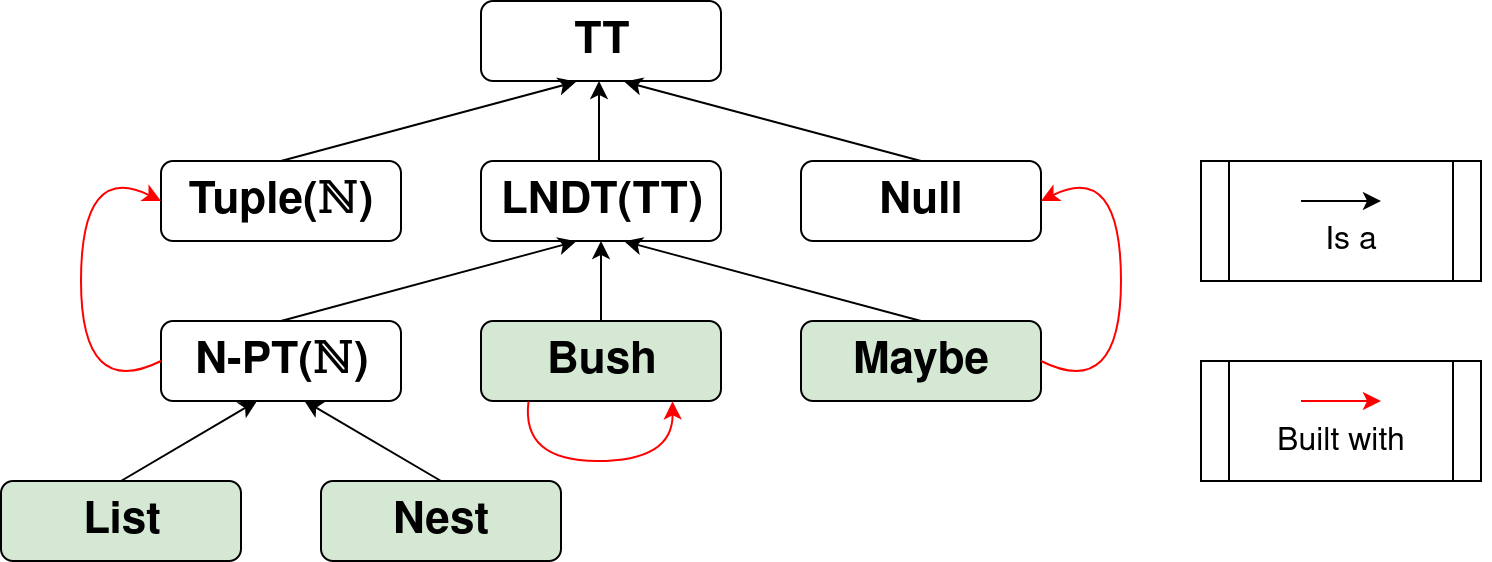
\includegraphics[width=.8\textwidth]{type-transformers}
\caption{Type transformers in \textsc{LibNDT}}
\label{overview}
\end{figure}

\section{Computational common behaviours}\label{sec:computational}

However tempting regrouping these types under a common denominator is, the relevance of this process depends on the possibility to express behaviours at the \linear level which could then be instantiated to any of its instances. The remaining of this paper stands as a list of argument in favour of this relevance, that is, a list of behaviours that can indeed be expressed for \linears. Such behaviours will be regrouped into 2 classes: computational ones, that is functions that affect the content of \linears, and logical ones, that is properties either directly bound to \linears or functions that work on them. In other words, the first class contains functions that process elements from \linears while the second class contains everything else. This section depicts our results regarding the first class of common behaviours.

When considering functions that work on collections of elements, a few examples come to mind, the first of which often is the \textit{map} primitive. The reasoning behind \textit{map} is well-known and natural: provided it is possible, using a certain function \texttt{f}, to transform elements of type \texttt{A} to elements of types \texttt{B}, it should be possible to transform a collection of elements of type \texttt{A} to a collection of elements of type \texttt{B} through a procedure, parametrized by \texttt{f}, called \textit{map}. We begin by studying the relevance of this assumption for \linears.

\subsection{Mapping \linears}\label{ssec:maps}

\myfirstparagraph{Building map functions for \linears} As this is our first example of common behaviour, let us consider, in details, the steps in our reasoning. Since lists are the simplest example of \linear we can start by considering the \textit{map} function written on lists.

\listmap

This is the common definition of maps for lists, which bears no noticeable difficulties. Writing a similar function for nests is somewhat more challenging because the tail of the nest is not of the same type of the nest itself, which means the same function \texttt{f} cannot be passed as it is in the recursive call.

\nestmap

However different, these two have a lot in common, which can be captured using \linears, as long as the way the function f must be transformed throughout the recursion is provided. By taking as parameter this transformation of function, and calling it \texttt{T}, we propose the following implementation for \linears.

\lndtmapz

While the signature of this function is not straightforward, it is possible to make it clearer by noticing a certain regularity in its core, which can be made visible as follows:

\mappable

This definition gives an abstract signature to type transformers \texttt{F} for which it is possible, given a function from \texttt{A} to \texttt{B}, to build a function from \texttt{F A} to \texttt{F B} that is, a map function. Using this new notation, the map function over \linears has a far better looking -- and much more explicit -- signature.

\lndtmap

This definition, through this new signature, gives us an important insight as to what \texttt{lndtmap} stands for: it is a procedure that ensure it is possible to map on \linears provided it is possible to map over the type transformer on which they are build. This is the first property that justifies the spreadable aspect of this library: we study which elements can be transported from \texttt{F} to \texttt{LNDT F}, and \texttt{Map} as defined earlier is one of them.

\myparagraph{Instantiating map functions} In order to deduce map functions for \linears, all is needed is to define a map function for the TT on which they are based. The first function, which can be spread to the annotated \linear, is called the seed for the associated behaviour. In this case, the behaviour in question is the ability to map over a given type. Here is the map seed for tuples:

\tuplesmap

The definitions of maps for \linears are hence straightforward:

\lndtmaps

What is particularly interesting here is that the map function on bushes is recursively generated using itself, solely relying on \texttt{lndtmap} as a way of computing a result. In other words, the seeds for bushes will never have to be defined and any behaviour on bushes is always solely generated with the associated spreadable property.

\myparagraph{Examples of usage of map functions} Here are examples where we first define a list of natural numbers on which we map the successor function, after which we define a bush of natural numbers on which we apply the multiplication by two function.

\firstexample

 In both case, \texttt{refl} is a correctly typed term regarding the signature of the function, which means both sides of the equality are indeed the same. These examples are by no means a proof of correctness of \texttt{map} but rather a convincing argument if favour of our approach and definitions. They also show that working with bushes is completely possible in \agda, so long the termination checker is turned off for their definition. This can prove to be an issue, though, when trying to work in a safe manner -- note that \agda itself has a safe option which disallow a certain number of options such as turning off the termination checker. This means that the problem of termination will need to be addressed at some point, and has already been tackled in a few manners using for instance other definitions of bushes with indices. However, this is not the goal of this work to handle such termination issues. We propose a global notion from which different concrete types can be defined, including bushes, and the fact itself that it is possible to work with them is interesting per se.

\myparagraph{Back to squared lists} Squared lists are second degrees \linears, in the sense that they are built by a succession of two nestings. For such types. However, regardless of the number of successive nestings, we can provide a map function as long as the seed -- the original TT -- provides a map function itself. Here is the function in question for squared lists:

\lndtlistmap

As an example of usage of this newly created map function, we can apply a multiplication by two on all elements of the example squared lists defined in Section~\ref{ssec:morelndt}

\lndtlistmapexample

As shown in this example, nesting several times over a given TT does not alter our ability to provide free functions from the seed of the chain. Throughout this paper, more examples of spreadable behaviours will be given, all of which can be spread several times similarly. As a consequence, we will not explicitly go back to squared lists.

\subsection{Folding \linears}\label{ssec:folds}

Another common behaviour which can be defined over \linears directly are the fold operators, whether right or left. While we described the whole thought process behind the map operator, we will, from now on, only give the property that is spreadable and the associated definitions. Both folds are spreadable and can thus be transferred from \texttt{F} to \texttt{LNDT F}. Both folds share the same abstract type:

\fold

Then, assuming we can fold over the type parameter, we can propagate this fold to \linear in two different manner, left or right. Here is the left propagation:

\folds

As an example of fold on an inner TT, here is the left fold on tuples:

\foldtuples

This leads to the definition of folds for our \linears. Here are the left folds for bushes and nests, with the respective seeds the fold on tuples, and itself.

\foldsinstances

Here are examples of usage of these folds. In the first case, we concatenate the string from left to right in a nest, and in the second case, from right to left in a bush:

\foldsexamples

\subsection{Summary}\label{ssec:computationalsummary}

This section exhibited three spreadable elements, that can be built freely for \texttt{LNDT F} when they exist on \texttt{F}, these are the two folds, left and right, and the map function. These elements can be regrouped inside a structure which contains all spreadable properties, which we call \texttt{SpreadAble}, and which will be enriched with logical properties from the next section. From the current element, it is possible to build other functions directly, such as size (the number of elements contained in a specific structure) and flatten, returning a list of these elements. This has been done in the library, however not shown here.

\section{Logical one}\label{sec:logical}

\section{Agda, Coq, Induction}

Parler des principes d'induction, de la positivité, etc, Agsy, terminaison à mettre ici

\section{Conclusion}\label{sec:conclusion}

\mathieu{parler de coq à la carte}

\mathieu{parler de comment étendre notre approche, exemple de types non directement implémentables éventuellement, mais le tourner positivement}

%\section{A \coq and an \agda implementations}
%
%\amelie{Je ne suis pas sûr que nous avons besoin d'une section en entier, mais il faut réserver une place pour parler un peu de la bibliothèque, notamment des différences entre les 2 implémentations. Nous pouvons également conclure avec un tableau qui regroupe toutes les fonctions que nous avons. }
%
%\mathieu{Je crois que c'est un reliquat d'ancien plan, en effet}
%
%\section{To go further}
%
%Discussion autour d'autres manières de nester (avec 3 constructeurs par exemple). Quel est l'effort de preuve nécessaire ?
%
%\section{Autre}
%
%Voir pour la notion d'inxation : indexer le nombre d'imbrication du transformateur de type par n, pour prouver par exemple de la terminaison sur les bush, ou avec une appartenance puissance n, est-ce utile ? Dans quelle mesure ? Que gagne t on et que perd t on ? C'est à discuter et peut être à expliquer.
%
%\begin{itemize}
%    \item data List a = Nil $|$ Cons (a, List a)
%    \item List A $\approx$ Base (A, List A)
%    \item data Base a b = Nil ( ) $|$ Cons (a, b)
%    \item Nil () is a terminal object
%    \item $Base (X, Y) = 1 + X \times Y$ \\
%    with $A + B = \{inl~a~|~a \in A\} \cup \{inr~b~|~b \in B\}$  \\
%    and $A \times B = \{(a, b)~|~a \in A,~b \in B\}$
%    \item On the equation, it's something like $LN(P,A) = 1~+~(A~\times~LN(P,P(A)))$
%\end{itemize}

%\begin{tikzpicture}
	%\tikzset{node distance=5mm and -25mm}  %Caractéristiques sur les noeuds
	\begin{scope}[on background layer]
	  			
    	\node[boite coins ronds]  (a) {------------------ Datatypes ------------------};
    
    	\node[boite coins ronds,below left=of a] (b) {Non recursive datatypes};
    	\node[boite coins ronds,below right=of a] (c) {Recursive datatypes};
    			
    	\draw[grosse fleche] (a) -- (b);
    	\draw[grosse fleche] (a) -- (c);
    					
    	\node[boite coins ronds,below left=of c] (d) {Nested datatypes};
    	\node[boite coins ronds,below right=of c] (e) {Regular datatypes \\
    	- List \\
    	- Tree};
    		
    	\draw[grosse fleche] (c) -- (d);	
    	\draw[grosse fleche] (c) -- (e);
    	
    	\node[boite coins ronds,below left=of d] (f) 
    	  {Linear \\ - Pow};
    	\node[boite coins ronds,below right=of d] (g) 
    	  {Non linear \\ - Bush};
    	
    	\draw[grosse fleche] (d) -- (f);
	    \draw[grosse fleche] (d) -- (g);
	    
	\end{scope}
\end{tikzpicture}


\newpage

\bibliography{types2021}

%\appendix

\end{document}
